% CREATED BY DAVID FRISK, 2015
\chapter{Results }

\hspace{0.25cm}This section explores the computational results obtained from the implementation. An explanation of the results is attempted and further comparison plots with the experimental results is provided.The experimental results were obtained from \cite{exp}.The main objective of this section is provide plots to show the behaviour of PANS with changing $f_k$(input).


\hspace{0.25cm}Initially RANS simulations were performed on the same geometry and grid to get an idea of the lower limit of$f_k$. Based on that, a set of $f_k$ values were chosen for both coarse and fine grids. The results obtained from them is reported in this section. A contour plot of mean and instantaneous Velocities is first shown. Further, $f_k$(output) comparison contour plots are displayed. A comparison line plots comparing several mean quantities with the experimental values is provided later.

\hspace{0.25cm}The simulations were monitored by measuring the drag fluctuations around the cube. Figure \ref{fig:41} represents plots of such fluctuations. It can be observed that for a coarse grid with $f_k$=0.8, the fluctuations normalize after sometime and it just captures the vortex shedding(RANS behaviour). Contrary to that, with $f_k$=0.15 for a fine grid, it shows that PANS can also capture further fluctuations along with vortex shedding.

\begin{figure}[H]
\begin{minipage}[b]{0.5\linewidth}
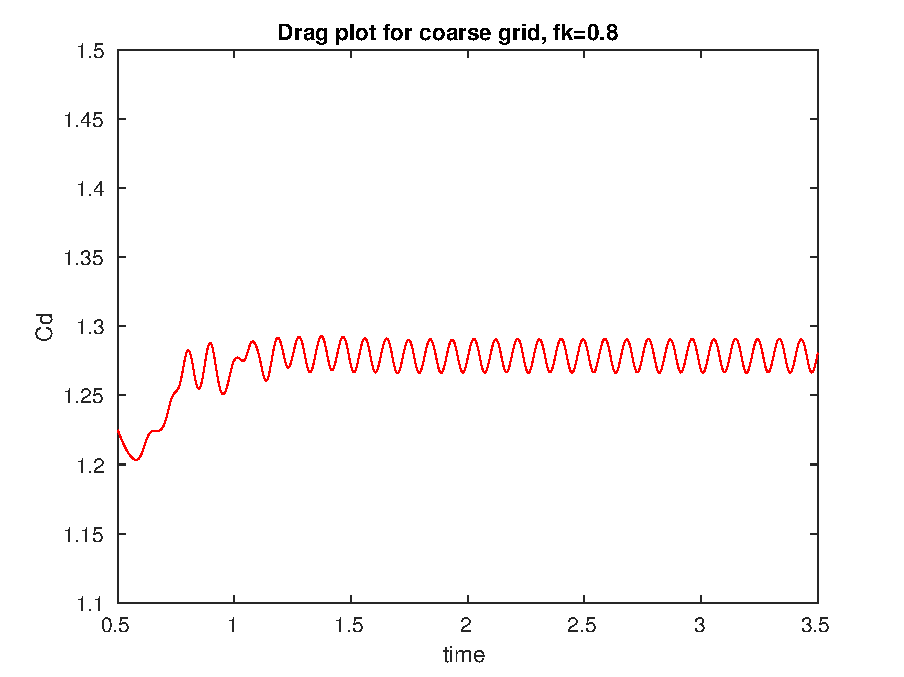
\includegraphics[scale=0.5]{figure/coarse/cd_coarse.pdf}
\end{minipage}
\begin{minipage}[b]{0.5\linewidth}
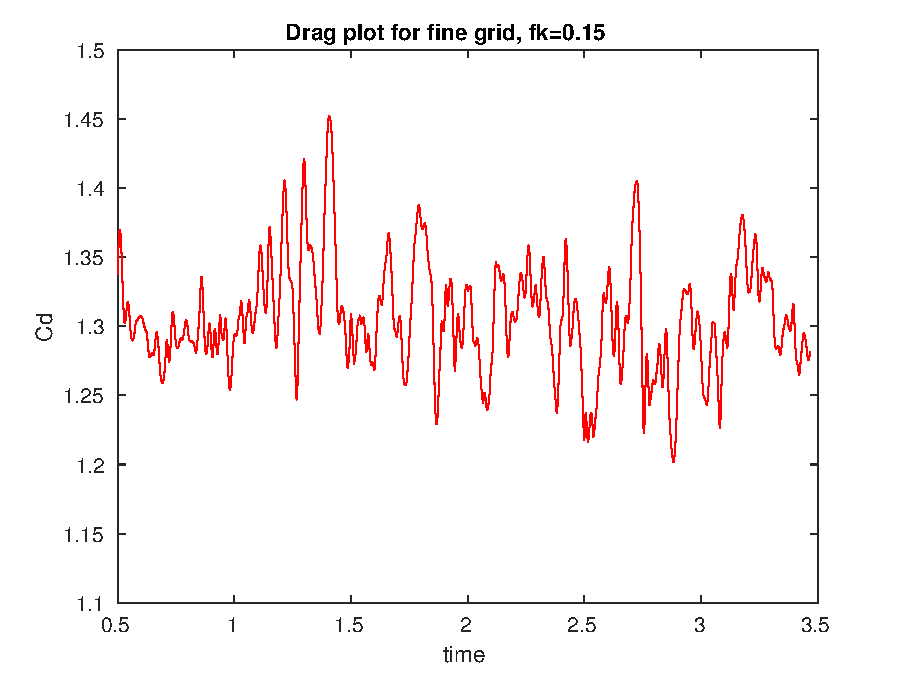
\includegraphics[scale=0.5]{figure/fine/cd_fine.pdf}
\end{minipage}
\caption{Drag fluctuations around the cube for coarse(left) and fine(right) grids}
\label{fig:41}
\end{figure}



\section{Mean Velocity Contour plots}

Figures \ref{fig:42} and \ref{fig:43} show the mean velocity plots along x direction for both coarse and fine grids. The simulations were averaged over 6 flow passes. The contour plots were obtained along the mid plane of the geometry. 


\begin{figure}[H]
\begin{minipage}[b]{0.5\linewidth}
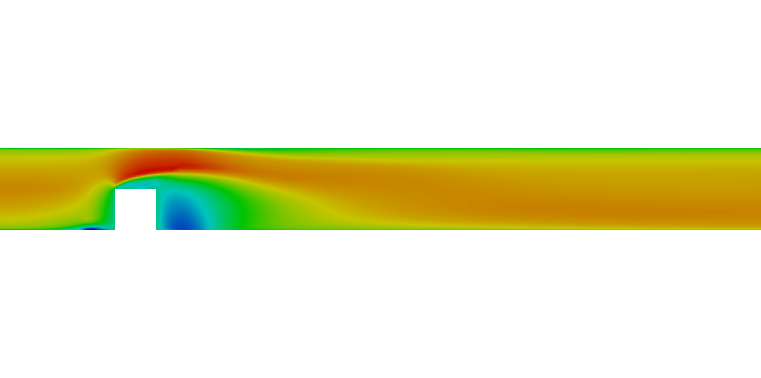
\includegraphics[scale=0.25]{figure/coarse/eight/Umean_z.png}
\caption*{$f_k$=0.8}
\end{minipage}
\begin{minipage}[b]{0.5\linewidth}
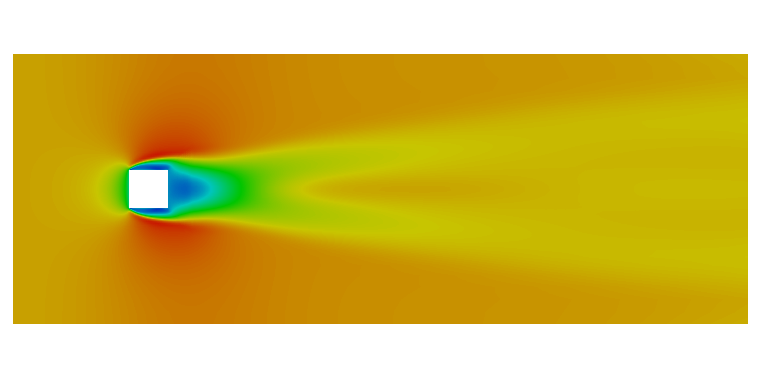
\includegraphics[scale=0.25]{figure/coarse/eight/Umean_y.png}
\caption*{}
\end{minipage}\\
\begin{minipage}[b]{0.5\linewidth}
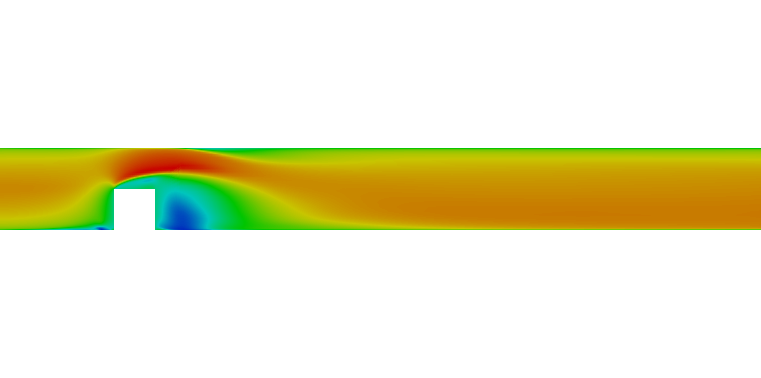
\includegraphics[scale=0.25]{figure/coarse/three/Umean_z.png}
\caption*{$f_k$=0.3}
\end{minipage}
\begin{minipage}[b]{0.5\linewidth}
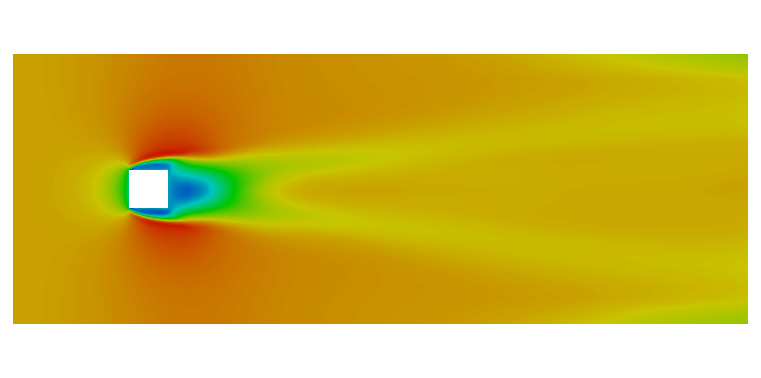
\includegraphics[scale=0.25]{figure/coarse/three/Umean_y.png}
\caption*{}
\end{minipage}\\
\begin{minipage}[b]{0.5\linewidth}
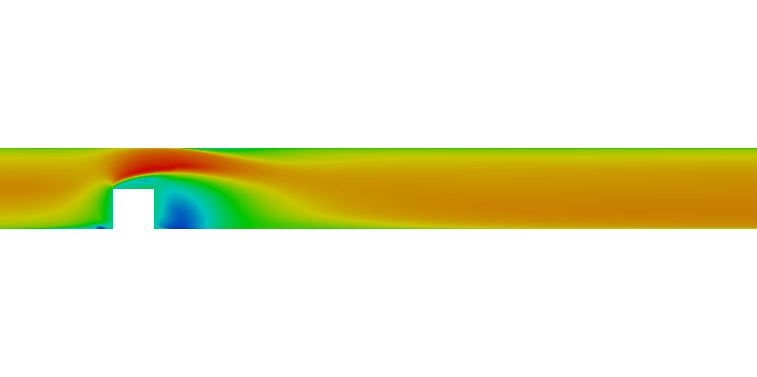
\includegraphics[scale=0.25]{figure/coarse/two/Umean_z.png}
\caption*{$f_k$=0.2}
\end{minipage}
\begin{minipage}[b]{0.5\linewidth}
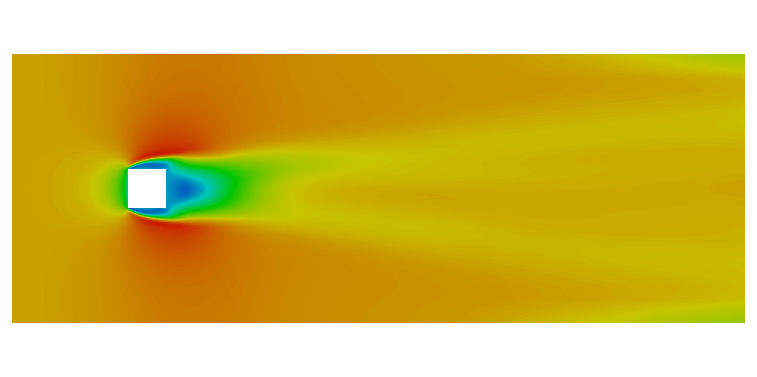
\includegraphics[scale=0.25]{figure/coarse/two/Umean_y.png}
\caption*{}
\end{minipage}\\
\begin{minipage}[b]{0.5\linewidth}
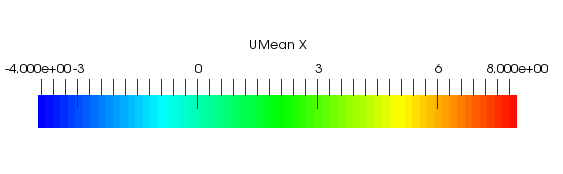
\includegraphics[scale=0.35]{figure/z_scale.png}
\end{minipage}
\begin{minipage}[b]{0.5\linewidth}
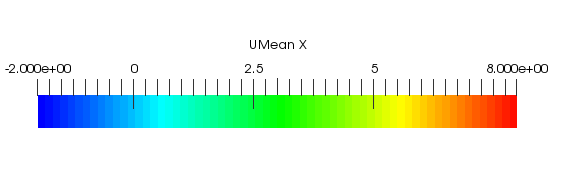
\includegraphics[scale=0.35]{figure/y_scale.png}
\end{minipage}\\

\caption{Mean velocity(U) plots about Z axis(left) and Y axis(right) for coarse grid}
\label{fig:42}
\end{figure}
\hspace{0.25cm}





\begin{figure}[H]
\begin{minipage}[b]{0.5\linewidth}
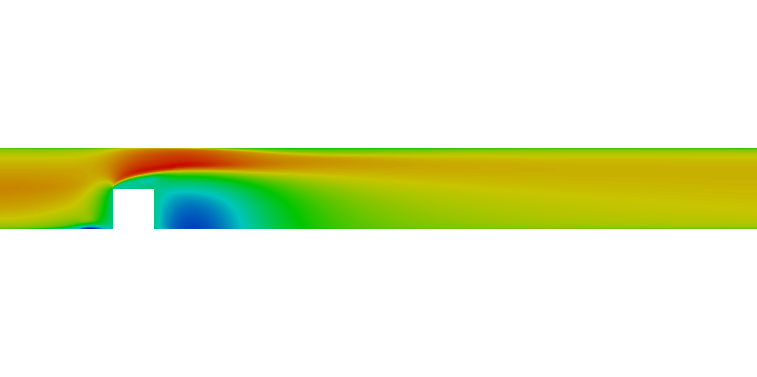
\includegraphics[scale=0.25]{figure/fine/eight/Umean_z.png}
\caption*{$f_k$=0.8}
\end{minipage}
\begin{minipage}[b]{0.5\linewidth}
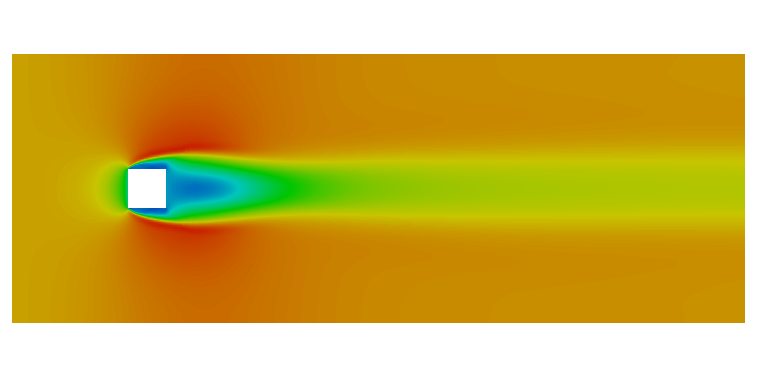
\includegraphics[scale=0.25]{figure/fine/eight/Umean_y.png}
\caption*{}
\end{minipage}\\
\begin{minipage}[b]{0.5\linewidth}
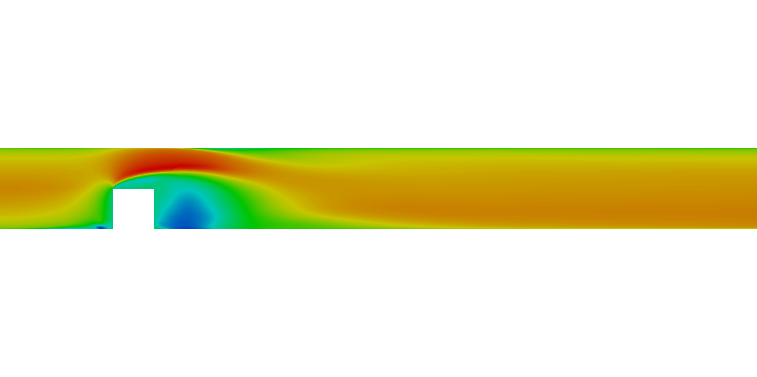
\includegraphics[scale=0.25]{figure/fine/three/Umean_z.png}
\caption*{$f_k$=0.3}
\end{minipage}
\begin{minipage}[b]{0.5\linewidth}
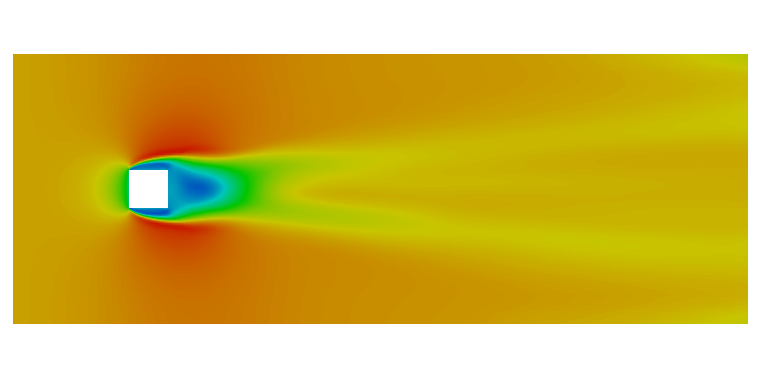
\includegraphics[scale=0.25]{figure/fine/three/Umean_y.png}
\caption*{}
\end{minipage}\\
\begin{minipage}[b]{0.5\linewidth}
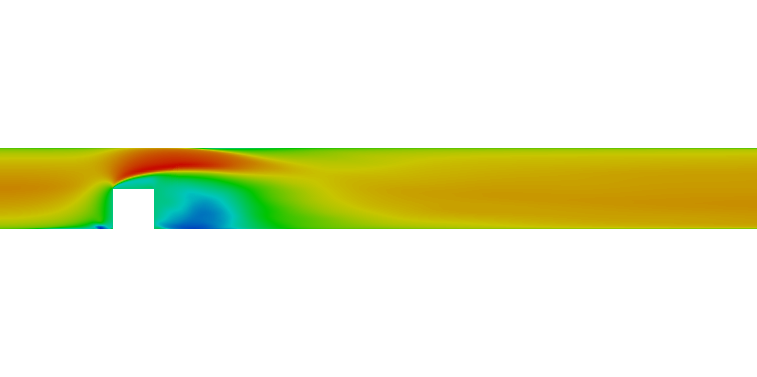
\includegraphics[scale=0.25]{figure/fine/one/Umean_z.png}
\caption*{$f_k$=0.15}
\end{minipage}
\begin{minipage}[b]{0.5\linewidth}
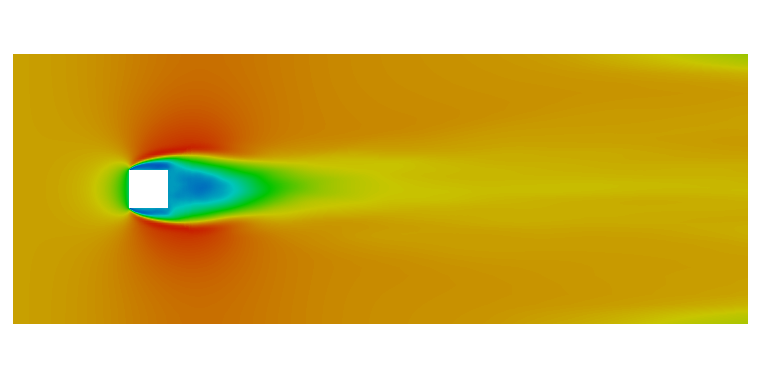
\includegraphics[scale=0.25]{figure/fine/one/Umean_y.png}
\caption*{}
\end{minipage}
\begin{minipage}[b]{0.5\linewidth}
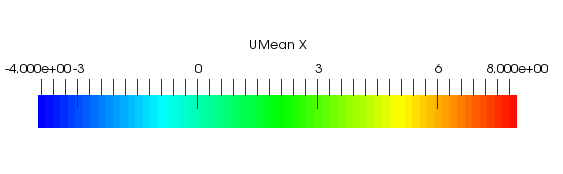
\includegraphics[scale=0.35]{figure/z_scale.png}
\end{minipage}
\begin{minipage}[b]{0.5\linewidth}
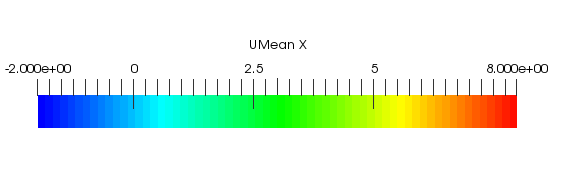
\includegraphics[scale=0.35]{figure/y_scale.png}
\end{minipage}\\

\caption{Mean velocity(U) plots about Z axis(left) and Y axis(right) for fine grid}
\label{fig:43}
\end{figure}


\section{Instantaneous Velocity Contour plots}



\begin{figure}[H]
\begin{minipage}[b]{0.5\linewidth}
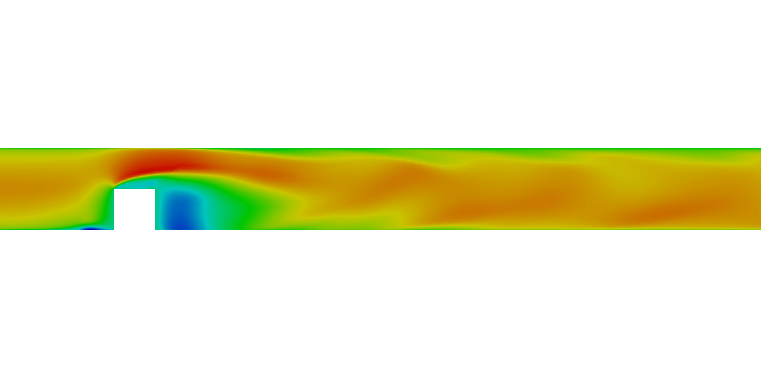
\includegraphics[scale=0.25]{figure/coarse/eight/Umag_z.png}
\caption*{$f_k$=0.8}
\end{minipage}
\begin{minipage}[b]{0.5\linewidth}
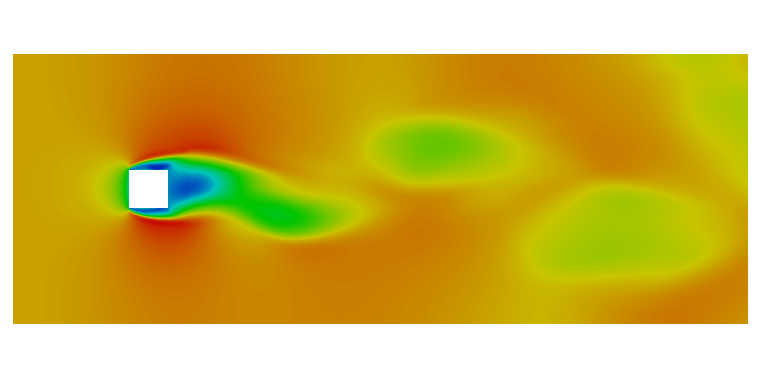
\includegraphics[scale=0.25]{figure/coarse/eight/Umag_y.png}
\caption*{}
\end{minipage}\\
\label{fig:eight}
\end{figure}
\newpage
\begin{figure}[H]
\ContinuedFloat
\begin{minipage}[b]{0.5\linewidth}
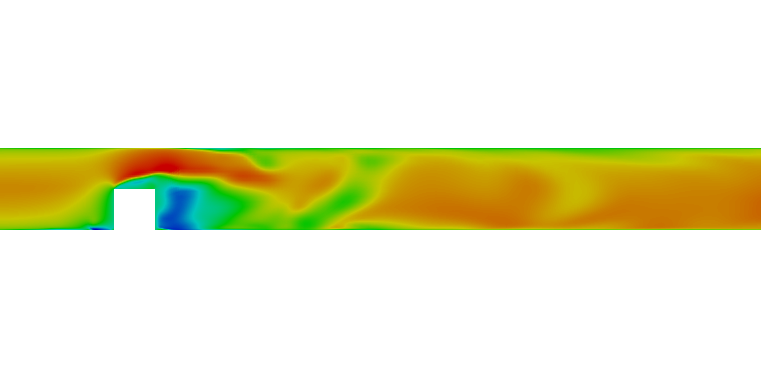
\includegraphics[scale=0.25]{figure/coarse/three/Umag_z.png}
\caption*{$f_k$=0.3}
\end{minipage}
\begin{minipage}[b]{0.5\linewidth}
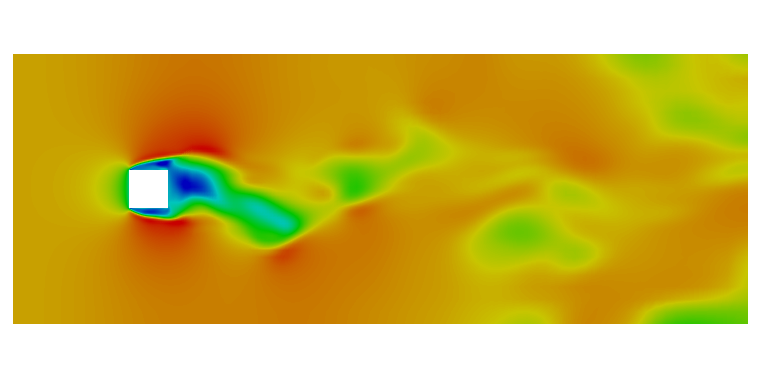
\includegraphics[scale=0.25]{figure/coarse/three/Umag_y.png}
\caption*{}
\end{minipage}\\

\begin{minipage}[b]{0.5\linewidth}
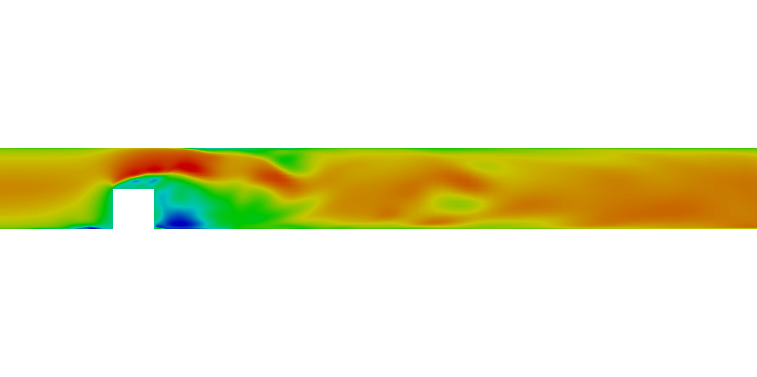
\includegraphics[scale=0.25]{figure/coarse/two/Umag_z.png}
\caption*{$f_k$=0.2}
\end{minipage}
\begin{minipage}[b]{0.5\linewidth}
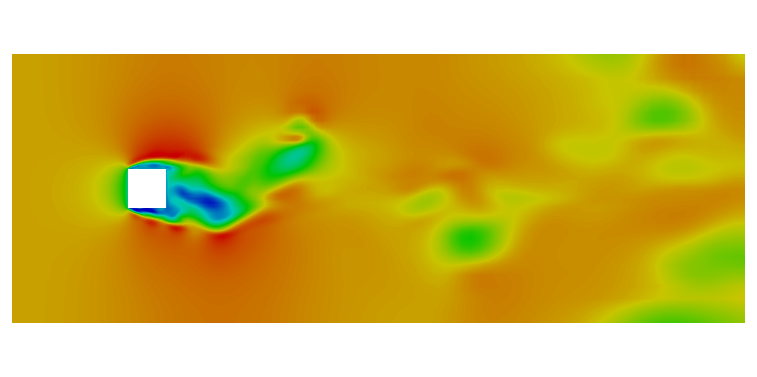
\includegraphics[scale=0.25]{figure/coarse/two/Umag_y.png}
\caption*{}
\end{minipage}
\begin{minipage}[b]{0.5\linewidth}
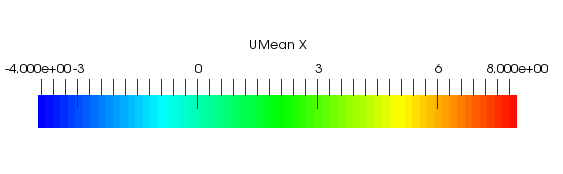
\includegraphics[scale=0.35]{figure/z_scale.png}
\end{minipage}
\begin{minipage}[b]{0.5\linewidth}
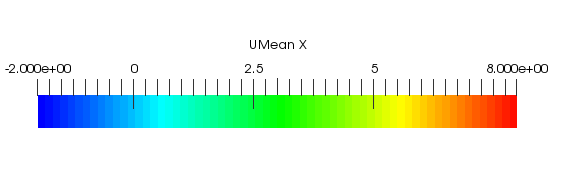
\includegraphics[scale=0.35]{figure/y_scale.png}
\end{minipage}\\
\caption{Instantaneous velocity(U) plots($t=4s$) about Z axis(left) and Y axis(right) for coarse grid}
\label{fig:43}
\end{figure}


Figures \ref{fig:43} and \ref{fig:44} give the instantaneous plots for U velocity at $t=4s$. The plots show the evolution of smaller flow structures with grid refinement and reducing $f_k$. 



\begin{figure}[H]
\begin{minipage}[b]{0.5\linewidth}
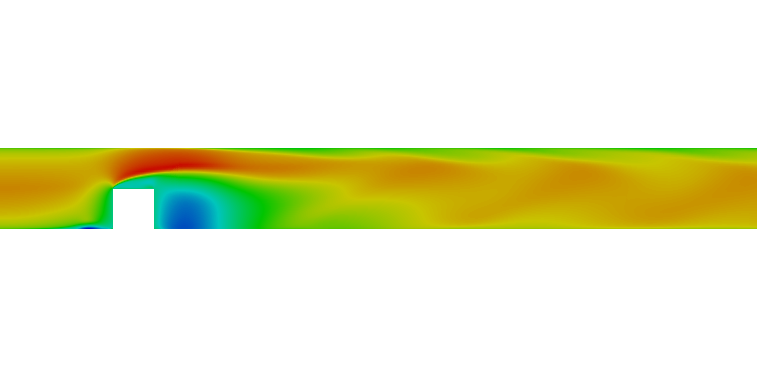
\includegraphics[scale=0.25]{figure/fine/eight/Umag_z.png}
\caption*{$f_k$=0.8}
\end{minipage}
\begin{minipage}[b]{0.5\linewidth}
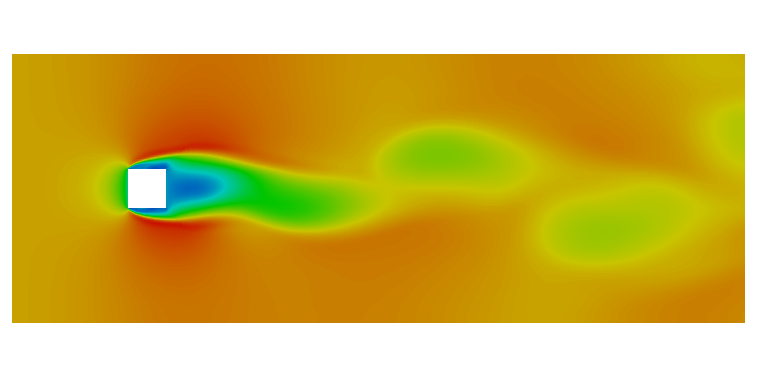
\includegraphics[scale=0.25]{figure/fine/eight/Umag_y.png}
\caption*{}
\end{minipage}\\
\caption{Instantaneous velocity(U) plots($t=4s$) about Z axis(left) and Y axis(right) for fine grid}
\label{fig:eight}
\end{figure}
\begin{figure}[H]
\ContinuedFloat
\begin{minipage}[b]{0.5\linewidth}
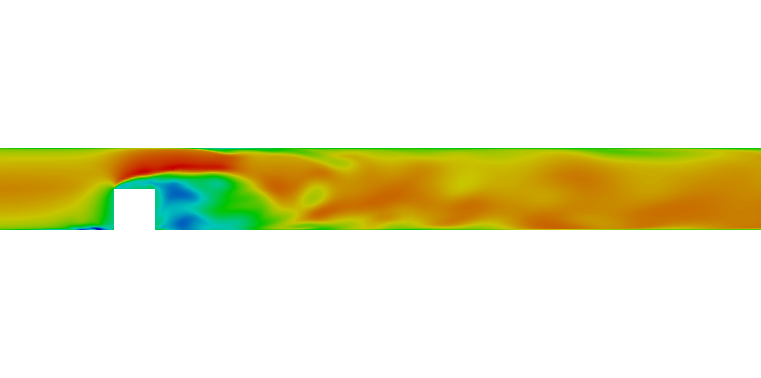
\includegraphics[scale=0.25]{figure/fine/three/Umag_z.png}
\caption*{$f_k$=0.3}
\end{minipage}
\begin{minipage}[b]{0.5\linewidth}
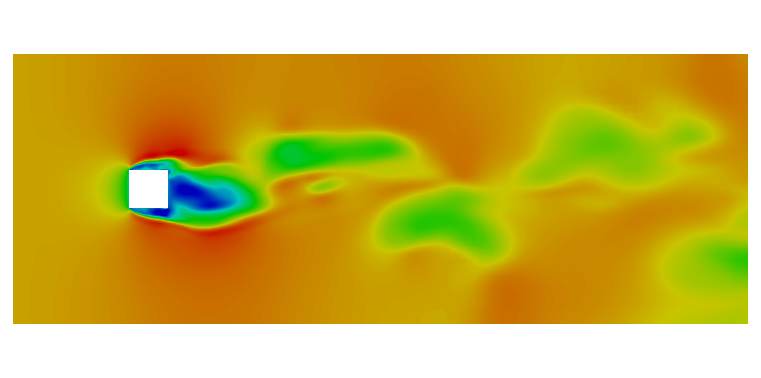
\includegraphics[scale=0.25]{figure/fine/three/Umag_y.png}
\caption*{}
\end{minipage}\\
\begin{minipage}[b]{0.5\linewidth}
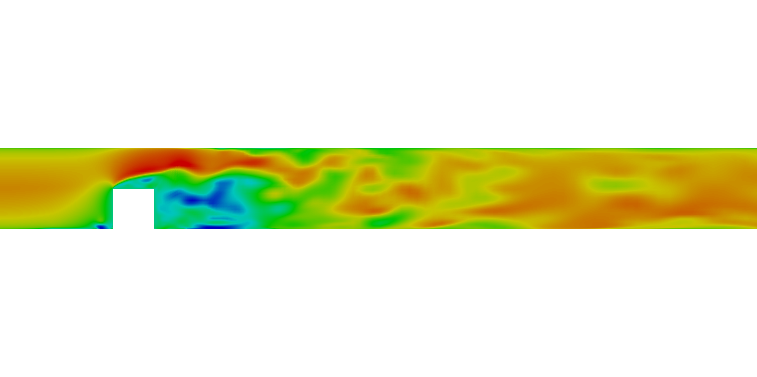
\includegraphics[scale=0.25]{figure/fine/one/Umag_z.png}
\caption*{$f_k$=0.15}
\end{minipage}
\begin{minipage}[b]{0.5\linewidth}
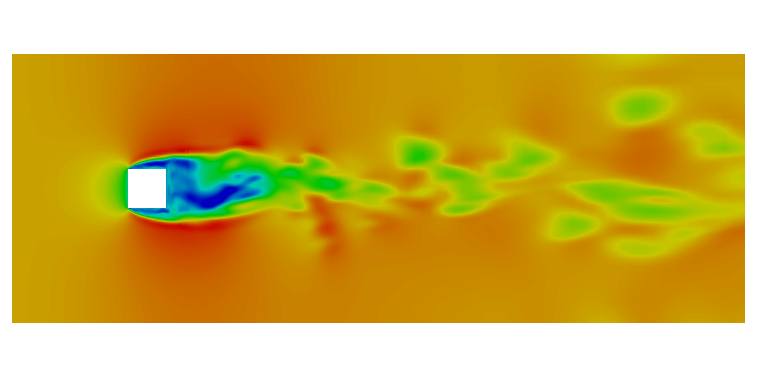
\includegraphics[scale=0.25]{figure/fine/one/Umag_y.png}
\caption*{}
\end{minipage}
\begin{minipage}[b]{0.5\linewidth}
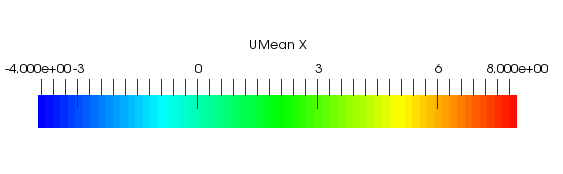
\includegraphics[scale=0.35]{figure/z_scale.png}
\end{minipage}
\begin{minipage}[b]{0.5\linewidth}
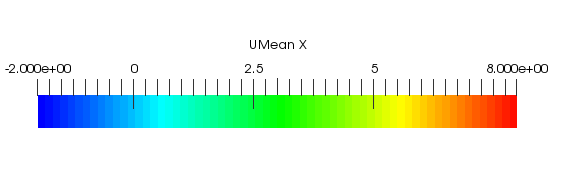
\includegraphics[scale=0.35]{figure/y_scale.png}
\end{minipage}\\
\caption{Instantaneous velocity(U) plots($t=4s$) about Z axis(left) and Y axis(right) for fine grid}
\label{fig:44}
\end{figure}



\section{Influence of $f_k$(input)}
Second invariant of velocity gradient $Q$, which is,  \(Q=-\frac{1}{2}(\frac{\partial u_i}{\partial x_j}\frac{\partial u_j}{\partial x_i})\) is an useful quantity in bluff body simulations to plot resolved flow structures. The term $u_i$ represents partially averaged velocity in PANS. The increasing capturing of smaller structures can be observed with the increase in both grid refinement and $f_k$(input).
\begin{figure}[H]
\begin{minipage}[b]{0.5\linewidth}
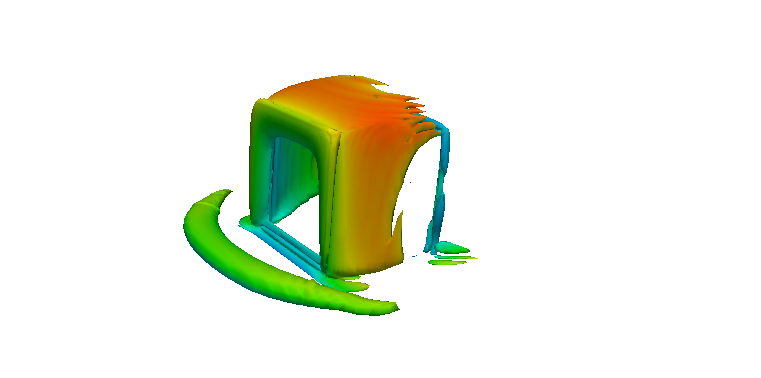
\includegraphics[scale=0.25]{figure/coarse/eight/iso.png}
\caption*{$f_k$=0.8}
\end{minipage}
\begin{minipage}[b]{0.5\linewidth}
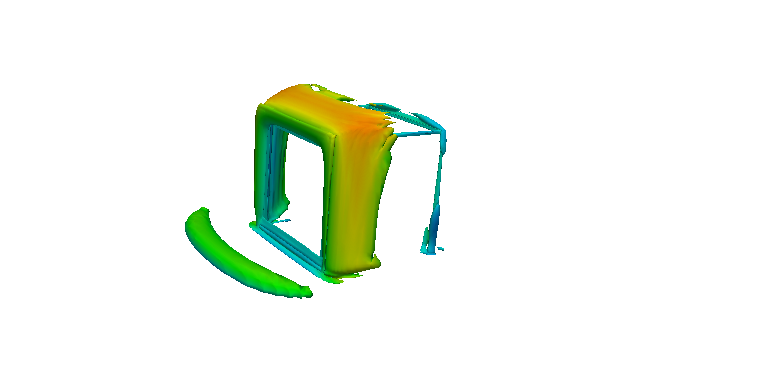
\includegraphics[scale=0.25]{figure/fine/eight/iso.png}
\caption*{$f_k$=0.8}
\end{minipage}\\
\caption{Iso-surface of Q-criterion coloured by Mean velocity(U) for coarse(left) and fine(right)}
\end{figure}
\begin{figure}[H]
\ContinuedFloat
\begin{minipage}[b]{0.5\linewidth}
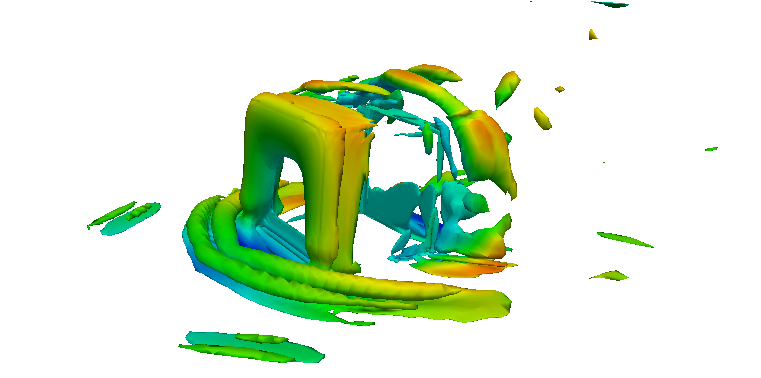
\includegraphics[scale=0.25]{figure/coarse/three/iso.png}
\caption*{$f_k$=0.3}
\end{minipage}
\begin{minipage}[b]{0.5\linewidth}
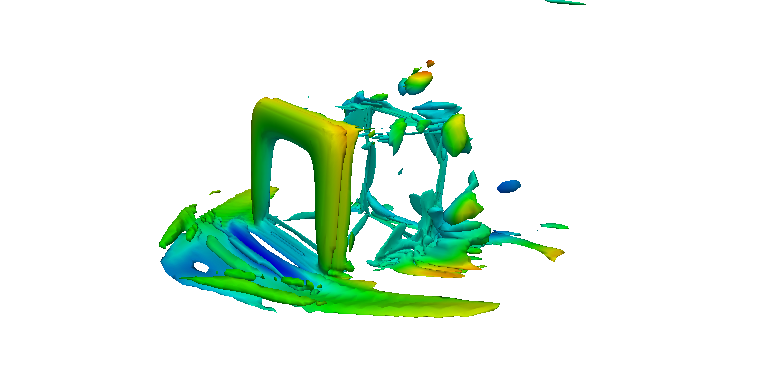
\includegraphics[scale=0.25]{figure/fine/three/iso.png}
\caption*{$f_k$=0.3}
\end{minipage}\\
\begin{minipage}[b]{0.5\linewidth}
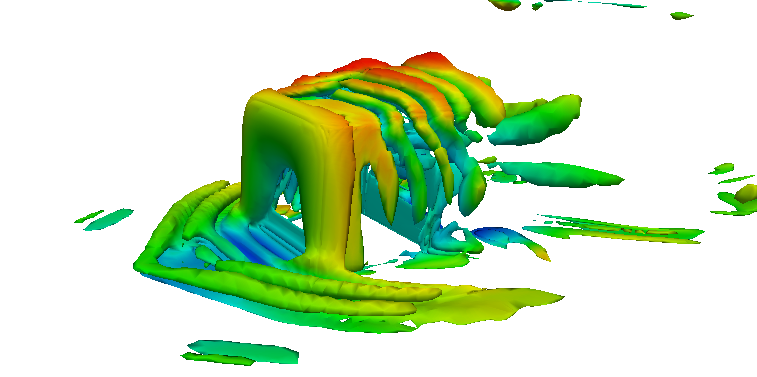
\includegraphics[scale=0.25]{figure/coarse/two/iso.png}
\caption*{$f_k$=0.2}
\end{minipage}
\begin{minipage}[b]{0.5\linewidth}
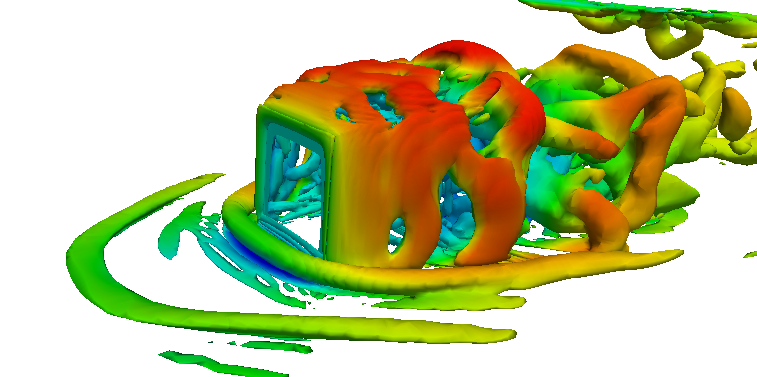
\includegraphics[scale=0.25]{figure/fine/one/iso.png}
\caption*{$f_k$=0.15}
\end{minipage}
\begin{center}
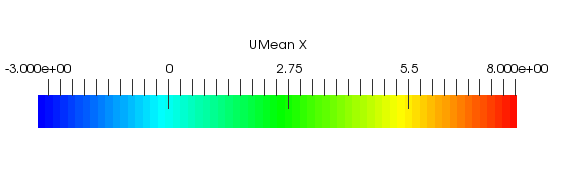
\includegraphics[scale=0.5]{figure/iso_scale.png}
\end{center}
\caption{Iso-surface of Q-criterion coloured by Mean velocity(U) for coarse(left) and fine(right)}
\end{figure}


\begin{comment}
\begin{figure}[H]
\begin{minipage}[b]{0.5\linewidth}
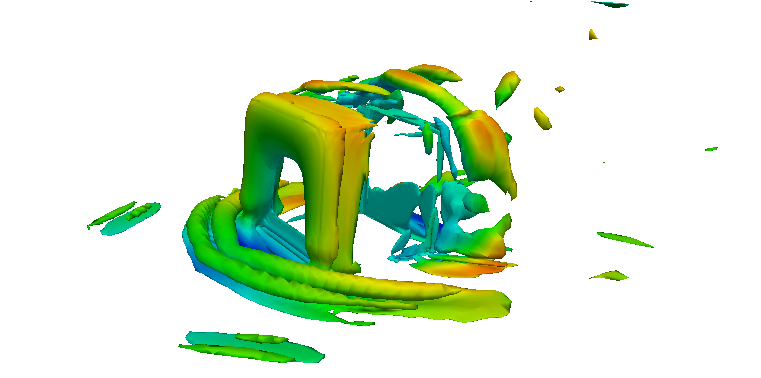
\includegraphics[scale=0.25]{figure/coarse/three/iso.png}
\end{minipage}
\begin{minipage}[b]{0.5\linewidth}
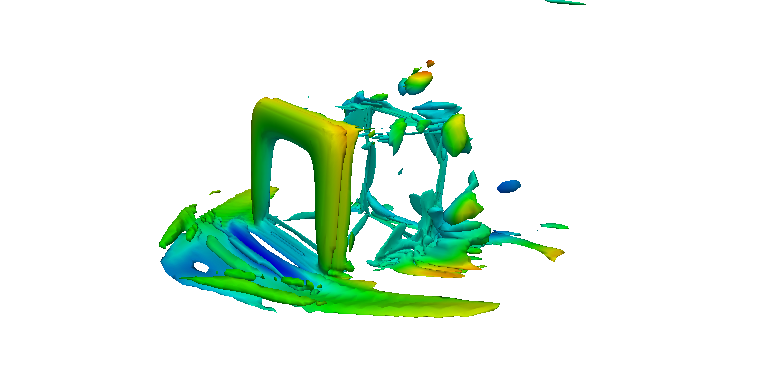
\includegraphics[scale=0.25]{figure/fine/three/iso.png}
\end{minipage}
\caption{Iso-surface of Q-criterion coloured by Mean velocity(U) for coarse(left, $f_k$=0.3) and fine(right, $f_k$=0.3)}
\end{figure}

\begin{figure}[H]
\begin{minipage}[b]{0.5\linewidth}
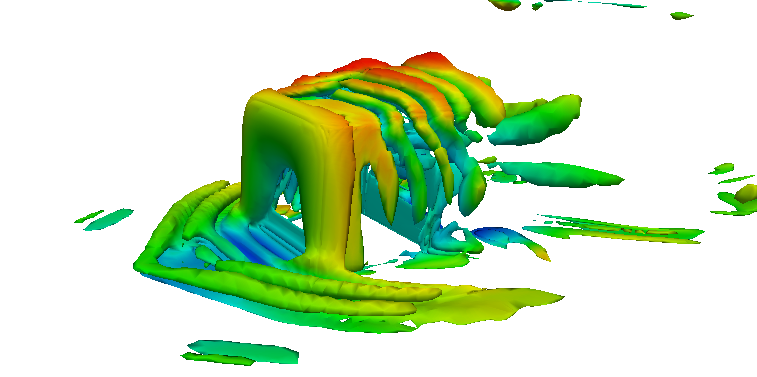
\includegraphics[scale=0.25]{figure/coarse/two/iso.png}
\end{minipage}
\begin{center}
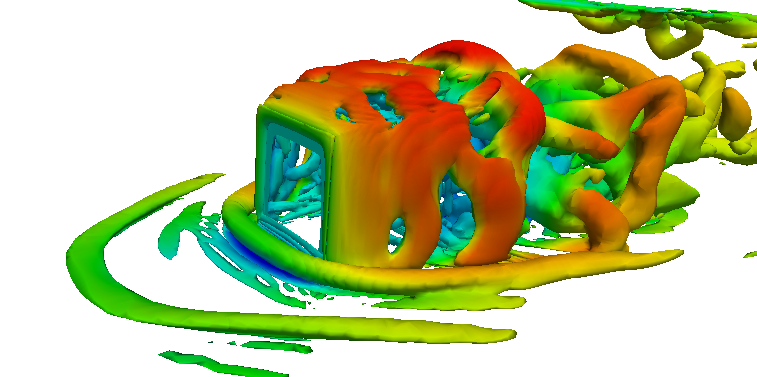
\includegraphics[scale=0.25]{figure/fine/one/iso.png}
\end{center}
\caption{Iso-surface of Q-criterion coloured by Mean velocity(U) for coarse(left, $f_k$=0.2) and fine(right, $f_k$=0.15)}
\end{figure}
\end{comment}

\section{$f_k$(output) plots}
\hspace{0.25cm}Figures \ref{fig:46} and \ref{fig:47} represent the influence of grid refinement and changing $f_k$(input) on $f_k$(output). It can be observed that the structures are more resolved with increasing grid refinement. 

\begin{figure}[H]
\begin{minipage}[b]{0.5\linewidth}
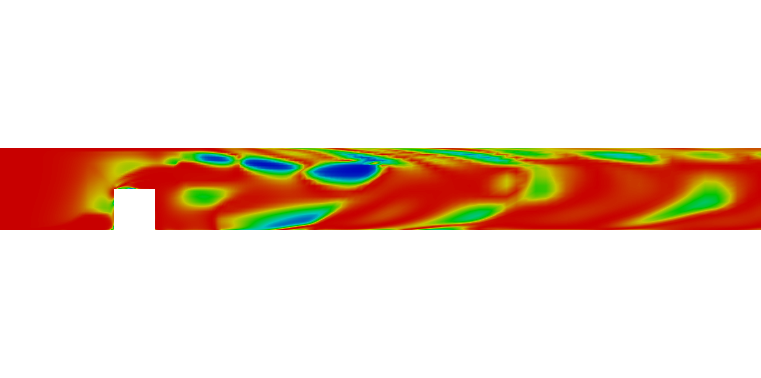
\includegraphics[scale=0.25]{figure/coarse/eight/fkout_z.png}
\caption*{$f_k$=0.8}
\end{minipage}
\begin{minipage}[b]{0.5\linewidth}
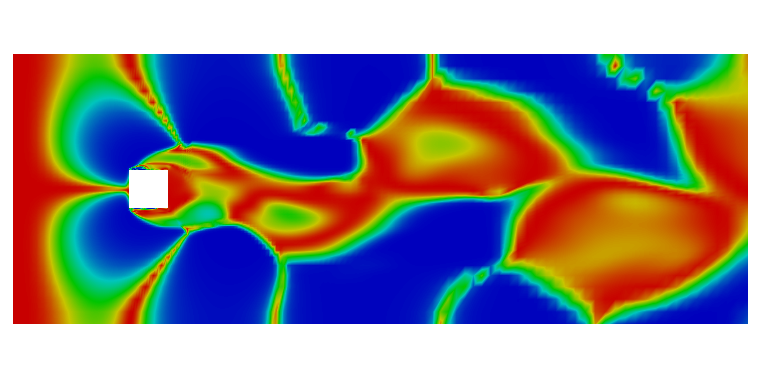
\includegraphics[scale=0.25]{figure/coarse/eight/fkout_y.png}
\caption*{}
\end{minipage}\\
\caption{$f_k$(output) plots about Z axis(left) and Y axis(right) for coarse grid}
\label{fig:eight}
\end{figure}

\begin{figure}[H]
\ContinuedFloat
\begin{minipage}[b]{0.5\linewidth}
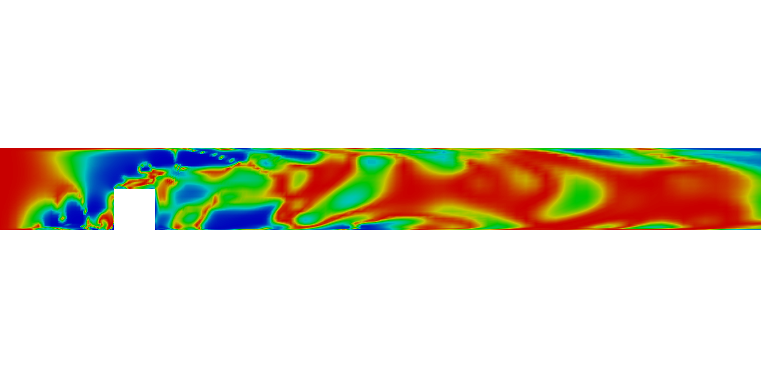
\includegraphics[scale=0.25]{figure/coarse/three/fkout_z.png}
\caption*{$f_k$=0.3}
\end{minipage}
\begin{minipage}[b]{0.5\linewidth}
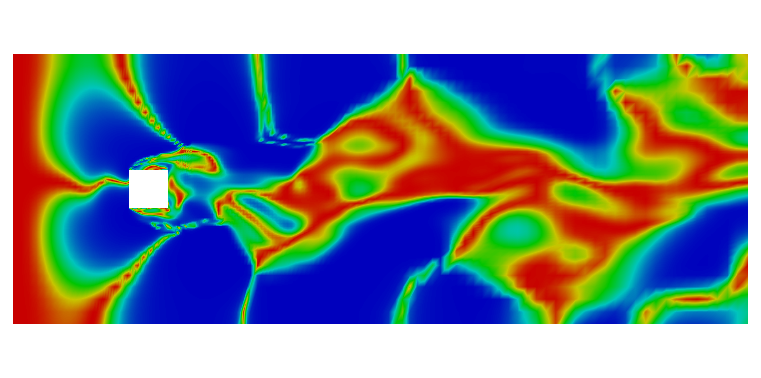
\includegraphics[scale=0.25]{figure/coarse/three/fkout_y.png}
\caption*{}
\end{minipage}\\
\begin{minipage}[b]{0.5\linewidth}
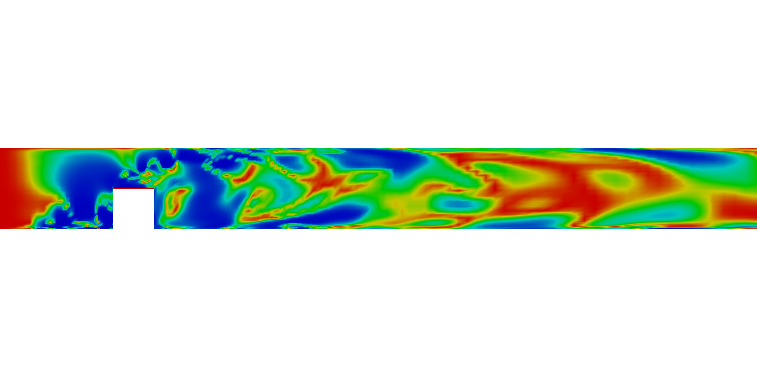
\includegraphics[scale=0.25]{figure/coarse/two/fkout_z.png}
\caption*{$f_k$=0.2}
\end{minipage}
\begin{minipage}[b]{0.5\linewidth}
\includegraphics[scale=0.25]{figure/coarse/two/fkout_y.png}
\caption*{}
\end{minipage}
\begin{center}
\includegraphics[scale=0.5]{figure/fk_scale.png}
\end{center}
\caption{$f_k$(output) plots about Z axis(left) and Y axis(right) for coarse grid}
\label{fig:46}
\end{figure}
On the higher spectrum of $f_k$, the results tend to be very dissipative. This could be because of the k-$\omega$ turbulence model is generally dissipative. But it seems to follow the flow pattern and resolve in important regions in the flow. Also, it can be observed through $f_k$(ouput) plots that more structures are released with increasing grid refinement and $f_k$(input).




 
\begin{figure}[H]
\begin{minipage}[b]{0.5\linewidth}
\includegraphics[scale=0.25]{figure/fine/eight/fkout_z.png}
\caption*{$f_k$=0.8}
\end{minipage}
\begin{minipage}[b]{0.5\linewidth}
\includegraphics[scale=0.25]{figure/fine/eight/fkout_y.png}
\caption*{}
\end{minipage}\\
\caption{$f_k$(output) plots about Z axis(left) and Y axis(right) for fine grid}
\label{fig:eight}
\end{figure}
\begin{figure}[H]
\ContinuedFloat
\begin{minipage}[b]{0.5\linewidth}
\includegraphics[scale=0.25]{figure/fine/three/fkout_z.png}
\caption*{$f_k$=0.3}
\end{minipage}
\begin{minipage}[b]{0.5\linewidth}
\includegraphics[scale=0.25]{figure/fine/three/fkout_y.png}
\caption*{}
\end{minipage}\\
\begin{minipage}[b]{0.5\linewidth}
\includegraphics[scale=0.25]{figure/fine/one/fkout_z.png}
\caption*{$f_k$=0.15}
\end{minipage}
\begin{minipage}[b]{0.5\linewidth}
\includegraphics[scale=0.25]{figure/fine/one/fkout_y.png}
\caption*{}
\end{minipage}
\begin{center}
 \includegraphics[scale=0.5]{figure/fk_scale.png}
\end{center}
\caption{$f_k$(output) plots about Z axis(left) and Y axis(right) for fine grid}
\label{fig:47}
\end{figure}



\section{Line plots}
A study of different line plots at locations, \(\frac{x}{H}=0.5\) and \(\frac{x}{H}=2\). The obtained results are compared with the experimental results. 

\begin{figure}[H]
\begin{minipage}[b]{0.5\linewidth}
\includegraphics[scale=0.5]{figure/coarse/U_coarse_five.pdf}
\end{minipage}
\begin{minipage}[b]{0.5\linewidth}
\includegraphics[scale=0.5]{figure/fine/U_fine_five.pdf}
\end{minipage}\\
\caption{Mean velocity(U) profile for coarse(left) and fine(right) grids}
\label{fig:eight}
\end{figure}
\begin{figure}[H]
\ContinuedFloat
\begin{minipage}[b]{0.5\linewidth}
\includegraphics[scale=0.5]{figure/coarse/U_coarse_two.pdf}
\end{minipage}
\begin{minipage}[b]{0.5\linewidth}
\includegraphics[scale=0.5]{figure/fine/U_fine_two.pdf}
\end{minipage}
\caption{Mean velocity(U) profile for coarse(left) and fine(right) grids}
\label{fig:48}
\end{figure}

\begin{comment}
\begin{figure}[H]
\begin{minipage}[b]{0.5\linewidth}
\includegraphics[scale=0.5]{figure/coarse/U_coarse_two.pdf}
\end{minipage}
\begin{minipage}[b]{0.5\linewidth}
\includegraphics[scale=0.5]{figure/fine/U_fine_two.pdf}
\end{minipage}
\caption{Mean velocity(U) profile for coarse(left) and fine(right) grids}
\label{fig:eight}
\end{figure}

\end{comment}
Both the U and V plots seem to be in close agreement with the experimental results apart from the V plot for the fine grid at \(\frac{x}{H}=2\) in figure \ref{fig:49}. It can also be observed in figure \ref{fig:48} for coarse grid at \(\frac{x}{H}=0.5\), $f_k$(input) of 0.8 performs better than others. The reason for this could be usage of a higher value of $f_k$(input) seems unnecessary for the coarse grid.

\begin{figure}[H]
\begin{minipage}[b]{0.5\linewidth}
\includegraphics[scale=0.5]{figure/coarse/V_coarse_five.pdf}
\end{minipage}
\begin{minipage}[b]{0.5\linewidth}
\includegraphics[scale=0.5]{figure/fine/V_fine_five.pdf}
\end{minipage}\\
\begin{minipage}[b]{0.5\linewidth}
\includegraphics[scale=0.5]{figure/coarse/V_coarse_two.pdf}
\end{minipage}
\begin{minipage}[b]{0.5\linewidth}
\includegraphics[scale=0.5]{figure/fine/V_fine_two.pdf}
\end{minipage}
\caption{Mean velocity(V) profile for coarse(left) and fine(right) grids}
\label{fig:49}
\end{figure}


\begin{comment}
\begin{figure}[H]
\begin{minipage}[b]{0.5\linewidth}
\includegraphics[scale=0.5]{figure/coarse/V_coarse_two.pdf}
\end{minipage}
\begin{minipage}[b]{0.5\linewidth}
\includegraphics[scale=0.5]{figure/fine/V_fine_two.pdf}
\end{minipage}
\caption{Mean velocity(V) profile for coarse(left) and fine(right) grids}
\label{fig:eight}
\end{figure}
\end{comment}




\begin{figure}[H]
\begin{minipage}[b]{0.5\linewidth}
\includegraphics[scale=0.5]{figure/coarse/UU_coarse_five.pdf}
\end{minipage}
\begin{minipage}[b]{0.5\linewidth}
\includegraphics[scale=0.5]{figure/fine/UU_fine_five.pdf}
\end{minipage}\\
\begin{minipage}[b]{0.5\linewidth}
\includegraphics[scale=0.5]{figure/coarse/UU_coarse_two.pdf}
\end{minipage}
\begin{minipage}[b]{0.5\linewidth}
\includegraphics[scale=0.5]{figure/fine/UU_fine_two.pdf}
\end{minipage}
\caption{Normalized stress($<u^{'}u^{'}>$) profile for coarse(left) and fine(right) grids}
\label{fig:eight}
\end{figure}
Figures above represent the normalized resolved stresses at the above mentioned locations. It can be observed that with the increasing $f_k$(input) value more fluctuations is observed at the locations.

\begin{comment}
\begin{figure}[H]
\begin{minipage}[b]{0.5\linewidth}
\includegraphics[scale=0.5]{figure/coarse/UU_coarse_two.pdf}
\end{minipage}
\begin{minipage}[b]{0.5\linewidth}
\includegraphics[scale=0.5]{figure/fine/UU_fine_two.pdf}
\end{minipage}
\caption{Normalized stress($<u^{'}u^{'}>$) profile for coarse(left) and fine(right) grids}
\label{fig:eight}
\end{figure}

\end{comment}

\section{Conclusions}
PANS was implemented for k-$\omega$ turbulence model in OpenFOAM. PANS seems to capture the flow structures satisfactorily. PANS seamlessly varies between RANS and DNS as the results show. The obtained results were validated with experimental results and they seem to agree closely. 


\section{Future work}
The work shows that PANS can provide intermediate accuracy at intermediate costs. A more optimized method to obtain $f_k$(input) is required in order to efficiently solve industrial problems. In real time applications there are always time varying boundary conditions. Intuitively, it can be seen that there is a requirement of a dynamic $f_k$(input) required to accommodate for these changes. In order to achieve this, the governing equations of the closure models need to be changed to adapt to the changing $f_k$(input). Some of the line plots are not in good agreement with the experimental results. This could be due to numerical errors since the case was not tested with varying numerical schemes. Therefore, a study to investigate this could be performed in the future. 




































